\definecolor{dkgreen}{rgb}{0,0.6,0}
\definecolor{gray}{rgb}{0.5,0.5,0.5}
\definecolor{mauve}{rgb}{0.58,0,0.82}
\definecolor{gray}{rgb}{0.4,0.4,0.4}
\definecolor{darkblue}{rgb}{0.0,0.0,0.6}
\definecolor{lightblue}{rgb}{0.0,0.0,0.9}
\definecolor{cyan}{rgb}{0.0,0.6,0.6}
\definecolor{darkred}{rgb}{0.6,0.0,0.0}

\lstset{
  basicstyle=\ttfamily\footnotesize,
  columns=fullflexible,
  showstringspaces=false,
  numbers=left,                   % where to put the line-numbers
  numberstyle=\tiny\color{gray},  % the style that is used for the line-numbers
  stepnumber=1,
  numbersep=5pt,                  % how far the line-numbers are from the code
  backgroundcolor=\color{white},      % choose the background color. You must add \usepackage{color}
  showspaces=false,               % show spaces adding particular underscores
  showstringspaces=false,         % underline spaces within strings
  showtabs=false,                 % show tabs within strings adding particular underscores
  frame=none,                   % adds a frame around the code
  rulecolor=\color{black},        % if not set, the frame-color may be changed on line-breaks within not-black text (e.g. commens (green here))
  tabsize=2,                      % sets default tabsize to 2 spaces
  captionpos=b,                   % sets the caption-position to bottom
  breaklines=true,                % sets automatic line breaking
  breakatwhitespace=false,        % sets if automatic breaks should only happen at whitespace
  title=\lstname,                   % show the filename of files included with \lstinputlisting;
                                  % also try caption instead of title
  commentstyle=\color{gray}\upshape
}


\lstdefinelanguage{XML}
{
  morestring=[s][\color{mauve}]{"}{"},
  morestring=[s][\color{black}]{>}{<},
  morecomment=[s]{<?}{?>},
  morecomment=[s][\color{dkgreen}]{<!--}{-->},
  stringstyle=\color{black},
  identifierstyle=\color{lightblue},
  keywordstyle=\color{red},
  % morekeywords={xmlns,xsi,noNamespaceSchemaLocation,type,id,x,y,source,target,version,tool,transRef,roleRef,objective,eventually}% list your attributes here
}

\lstdefinelanguage{json}{}

\section{Dataset}
This section describe the chosen dataset and explain how we enriched it. Statistics about data are also presented.
\subsection{Initial Dataset}
\subsubsection{Description}
The first challenge we had to face was finding a corpus of movies' dialogues. Luckily, our supervisor provided us one called Movie-DiC. This corpus has been built by R. Banchs \cite{banchs} for research and development purposes.\\
Movie-DiC comprises 132,229 dialogues, containing 764,146 turns (also called utterances) extracted from 753 different movies. In \cite{banchs}, the author mention some basic statistics about the corpus :
\begin{itemize}
\item Avg. amount of dialogues per movie : 175.60
\item Avg. amount of utterances per dialogue : 5.78
\end{itemize}
The corpus consist on a XML document of 2,249,053 lines, its structure isn't so complex since his maximal depth is only of 3 (movie - dialogue - utterance). See Code~\ref{code:dial} for an example of a dialogue unit.\\
\lstinputlisting[language=XML,caption=Dialogue unit,label={code:dial}]{dialUnit.xml}
This dialogue is pulled out the \say{xXx} movie\footnote{xXx on IMDB : http://www.imdb.com/title/tt0295701/} produced in 2002 by Rob Cohen.
\subsubsection{Remarks}
This dataset is really interesting but some details rose small issues during the project.\\
First, as you can see above in Code~\ref{code:dial}, one dialogue is in fact a succession of tags which follows a specific patern :
\begin{enumerate}
\item Speaker : who is speaking ?
\item Mode : is he happy/suspicious/\dots ?
\item Context : description of the shot
\item Utterence : the speaker's speech
\end{enumerate}
We found it strange that all those 4 tags aren't childs of another one, let say \say{utterance}. It would make more sense given the XML spirit and would also be easier to parse. Here we had to iterate on the dialogue's childs and group every group of 4 tags together in a single entity.\\
Then, some of the movies' titles are modified. For instance \say{X Files Fight the Future The} in fact refers to the movie \say{The X Files Fight the Future}. These little modifications are a problem when it comes to the enrichments phase (see section~\ref{ssec:enrich}). \\
Finally, the XML document wasn't totally correct, there were special characters such as \say{\&} which blocked the python XML parser. A root tag was also missing.
\subsection{Enrichments}
\label{ssec:enrich}
The Movie-DiC corpus only contains data about the content of the movie, but no data about the movie itself apart from its title. In order to build statistics, presented in section \ref{ssec:stats}, we enriched the corpus with the help of the Open Movie Database (short OMDb) API\footnote{http://www.omdbapi.com/}. This API is maintained by its users and isn't endorsed by or affiliated with the more famous IMDB website\footnote{http://www.imdb.com/}.\\
The use of the OMDb is really simple. It provides a web service which allows us to search for a movie given its title. It then returns lot of data about the movie such as its released year/date, genre, director's and actor's names, language, country. It also pull out some data from imdb such as the number of votes or the average rating.\\
Here's an example of usage :\\
Query : http://www.omdbapi.com/?t=Whiplash\&plot=short\&r=json\\
Answer :
\lstinputlisting[language=json,caption=OMDb answer,label={code:omdb}]{whiplash.json}

\newpage
\subsection{Statistics}
\label{ssec:stats}

\paragraph{Motivation}
\label{par:Motivation}
The idea which lays behind these statistics is to get a better understanding of the data we added to the corpus.
In this section, we are going to stress our data, aggregate it, and try to extract some meaning.
We have no pretention to be cinema experts, and there are obvious bias to any statistics which would be built on this data :
\begin{itemize}
    \item First, we are working on a dataset which contains data about less than a thousand movies.
    This is a lot, but at the same time, this is very few, when you know that more than 1450 movies have had an international publication in 2014.
    \item The ratings we base our rankings on are the ratings of ImDB users. Users are not experts.
    Their ratings show how they feel about the movies, but they are not a proof (nor even a direct indicator) that a movie is good or bad.
\end{itemize}

\paragraph{Modus Operandi}
\label{par:ModusOperandi}
All the aggregated statistics you are going to see in this section are based on data aggregated on the condition that there is enough of it.
For instance, in the next section \ref{subs:Director}, we are going to describe which film directors have made the movies that were most (and least) appreciated by the public.
In order to avoid outliers, especially in such a small dataset, we decided not to evaluate the movies from directors of whom only one movie is represented.
This method is not perfect, and to have stronger results, we should have increased this threshold to 5 movies at least.
But the author of our dataset decided not to focus on some specific directors, and to represent as many of them as possible.

\subsubsection{Directors}
\label{subs:Directors}

Directors rankings that follow in Figures~\ref{fig:bestDirectors}~and~\ref{fig:worstDirectors} don't rate the talent of the directors mentioned.
They only represent how the ImDB users rated these directors' movies (the ones that are in our dataset, if there are at least two movies for each director in the dataset).
Although they are quite consistent with global directors' fame, we cannot help noticing that Brian de Palma, who is quite famous for movies such as \textit{Scarface} or \textit{The incorruptibles}, is ranked very poorly.
This is because, although his movies are famous, they are not always highly rated.
We could have expected the same from Steven Spielberg's movies, which are also quite mainstream, but the latter is, on the contrary, among the most successfull directors.
That's one downside of the movie sampling that was made to build this dataset.

\begin{figure}[!h]
\begin{center}
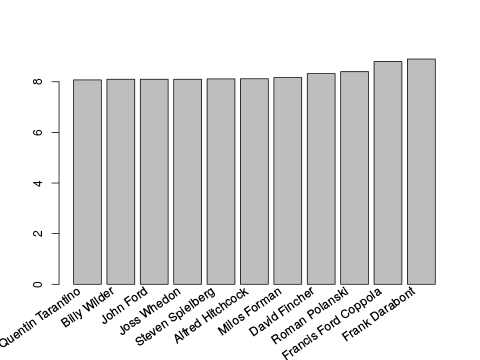
\includegraphics[width=0.70\textwidth]{../src/pre-processing/stats/results/bestDirectors.png}
\end{center}
\caption{Best directors}
\label{fig:bestDirectors}
\end{figure}

\begin{figure}[!h]
\begin{center}
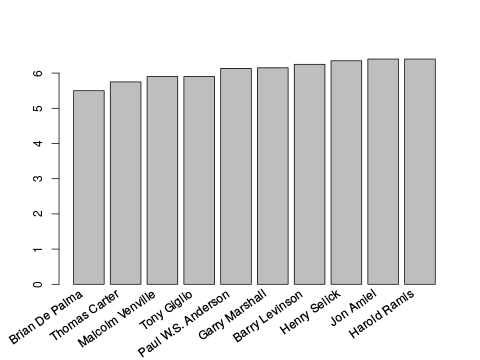
\includegraphics[width=0.70\textwidth]{../src/pre-processing/stats/results/worstDirectors.png}
\end{center}
\caption{Worst directors}
\label{fig:worstDirectors}
\end{figure}

\newpage
\subsubsection{Countries}
\label{subs:Countries}

For ranking countries (see Figure~\ref{fig:rateByCountry}), there is also one bias with sample size and representativity.
Besides, from one country to another, the standards are note the same, and we must keep in mind that ImDB is an American Website, with American members.
Not all Swedish movies are excellent, and not indian movies are mocked by the occidental readers of ImDB.

\begin{figure}[!h]
\begin{center}
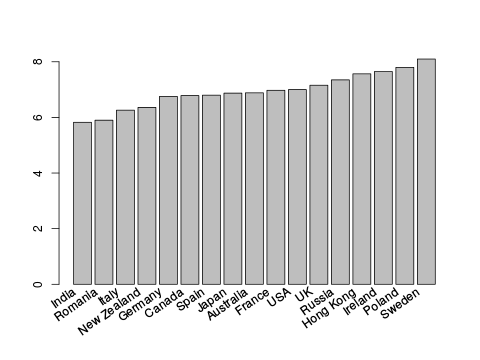
\includegraphics[width=0.70\textwidth]{../src/pre-processing/stats/results/rateByCountry.png}
\end{center}
\caption{Average movie rating for each country}
\label{fig:rateByCountry}
\end{figure}

One more interesting thing to measure is the interaction between countries in co-producing movies.
We can see that there is a large historical occidental cluster (USA, UK, France, Germany) around which the co-producing is articulated.
This is of course also a biased result, because most of the movies in the dataset are occidental ones.

\begin{figure}[!h]
\begin{center}
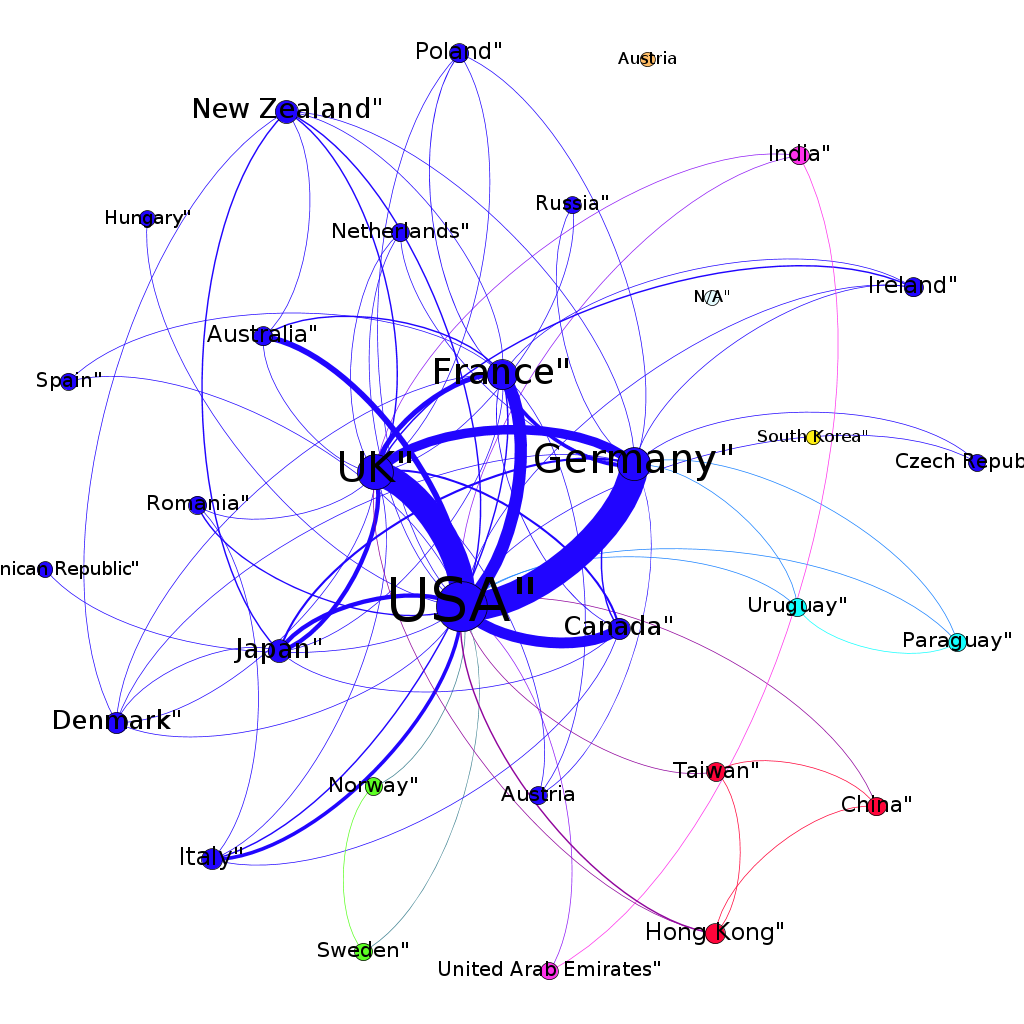
\includegraphics[width=0.7\textwidth]{../src/pre-processing/stats/results/CoocCountry.png}
\end{center}
\caption{Network of countries co-producing movies}
\label{fig:coocCountry}
\end{figure}

\subsubsection{Ratings}
\label{subs:Ratings}

Is \textit{the old better than the new} ? Not for movies, at least.
Although we would have expected some bias that would play in favour of old movies (Selection\footnote{The movies in this dataset were obviously selected for their diversity, but also for their quality : for an old movie not to be forgotten, it takes more than for a recent one.},
 \textit{Hipstering}, Quantity), it seems that the average rating is getting better with time (see Figure~\ref{fig:ratingEvolution})
How to interpret that ? Well, an interesting phenomenon is that when you look at the all-time best movies ranking on ImDB, the top movies are either very old, or, most of the time, very recent.
The very old thing can be explained by the combination of two phenomenon :
\begin{itemize}
    \item Quantity : there are more and more movies right now, with bigger and bigger budget.
    So, basically, now, everyone can make his own movie, and try and hide his lack of talent behind massive special effects or famous actors.
    \item Hipstering : for some reason, it is \textit{cool} to like old movies and to promote them as better than the recent blockbusters, which are so \textit{mainstream}.
\end{itemize}
On the other hand, the fact that recent movies are well rated can be explained with a more psychological approach : people tend to like what is new.
Besides, the novelty of a movie like \textit{Avatar} (J.Cameron, 2009) was the mind-blowing special effects, which seem now quite dipappointing, even though the critics were dithyrambic at the time.
For a movie to survive old-fashioned special effects, it takes talent (Confer the fist \textit{Star Wars} trilogy).
That's why recent blockbusters are often disavowed a few years later.

\begin{figure}[!h]
\begin{center}
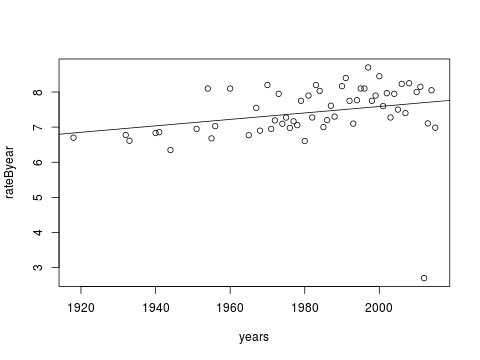
\includegraphics[width=0.70\textwidth]{../src/pre-processing/stats/results/ratingEvolution.png}
\end{center}
\caption{Evolution of rating over time}
\label{fig:ratingEvolution}
\end{figure}

Figure~\ref{fig:ratingPerNbVotes} is also quite interesting.
On the one hand, we could say that there is no direct correlation between the quality of a movie and the quantity of users that evaluated it,
because there are movies evaluated as good with few evaluations, and there are some with many\footnote{Although there are more with few than with many.}.
But on the other hand, movies rated as bad by ImDB users are never evaluated by many users.

\begin{figure}[!h]
\begin{center}
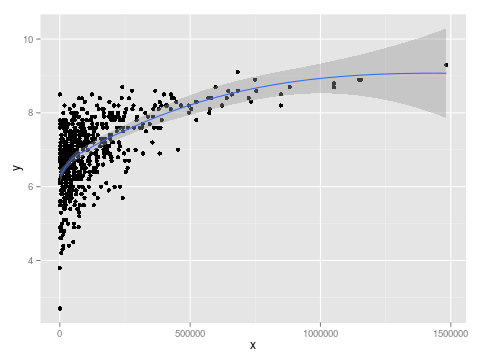
\includegraphics[width=0.70\textwidth]{../src/pre-processing/stats/results/ratingPerNbVotes.png}
\end{center}
\caption{Rating related to amount of ImDB users who voted}
\label{fig:ratingPerNbVotes}
\end{figure}

\newpage
Figure~\ref{fig:ratingPerRuntime} raises the issue of a correlation between rating and runtime.
Well, this is definitely not obvious.
By proceeding a simple least-square linear regression, we can say that the trend is for longer movies to be more appreciated.

\begin{figure}[!h]
\begin{center}
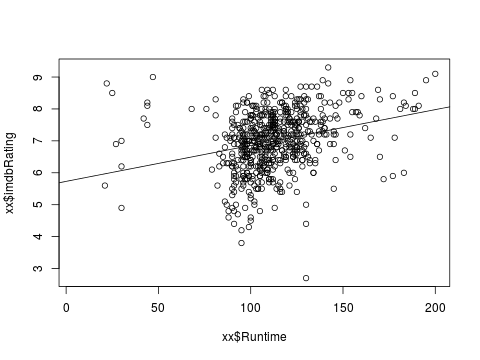
\includegraphics[width=0.70\textwidth]{../src/pre-processing/stats/results/ratingPerRuntime.png}
\end{center}
\caption{Rating related to film duration}
\label{fig:ratingPerRuntime}
\end{figure}

\newpage
\subsubsection{Genre}
\label{subs:Genre}

We can see in Figure~\ref{fig:rateByGenre} that usually, the best ratings are given to movies that deal with serious topics (\textit{History}, \textit{Biography}, \textit{War}).
On the other hand, large-audience topics, such as \textit{Horror} or \textit{Action} movies, or \textit{Comedies}, even though they are very popular, seem to be evaluated as less "good" by the audience.
One surprising result is that \textit{Documentaries} are unexpectedly low in this ranking, when the popular \textit{Drama} is quite high.

\begin{figure}[!h]
\begin{center}
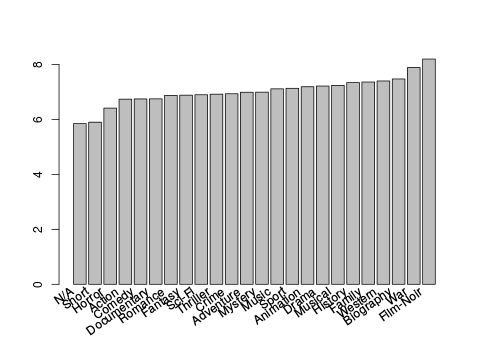
\includegraphics[width=0.70\textwidth]{../src/pre-processing/stats/results/rateByGenre.png}
\end{center}
\caption{Average movie rating for each genre}
\label{fig:rateByGenre}
\end{figure}

In Figure~\ref{fig:dureeByGenre}, we see that the ranking is quite similar as in Figure~\ref{fig:rateByGenre}.
The longer the better : that's a result we already saw in Figure~\ref{fig:ratingPerRuntime} where we evaluated the correlation between rating and duration.
Let's note, though, that most \textit{Films-Noirs} are shorter than the average, and still they get the best ratings.

\begin{figure}[!h]
\begin{center}
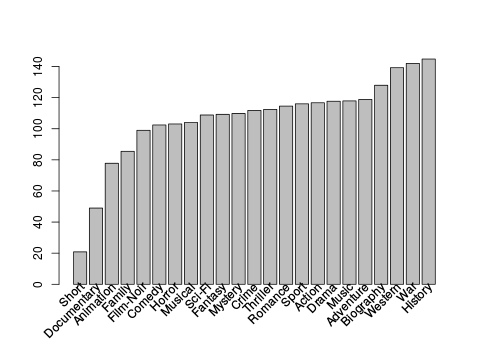
\includegraphics[width=0.75\textwidth]{../src/pre-processing/stats/results/dureeByGenre.png}
\end{center}
\caption{Average movie duration for each genre}
\label{fig:dureeByGenre}
\end{figure}

We can also study (see Figure~\ref{fig:coocGenre}) the proximity between the different genres.

\begin{figure}[!h]
\begin{center}
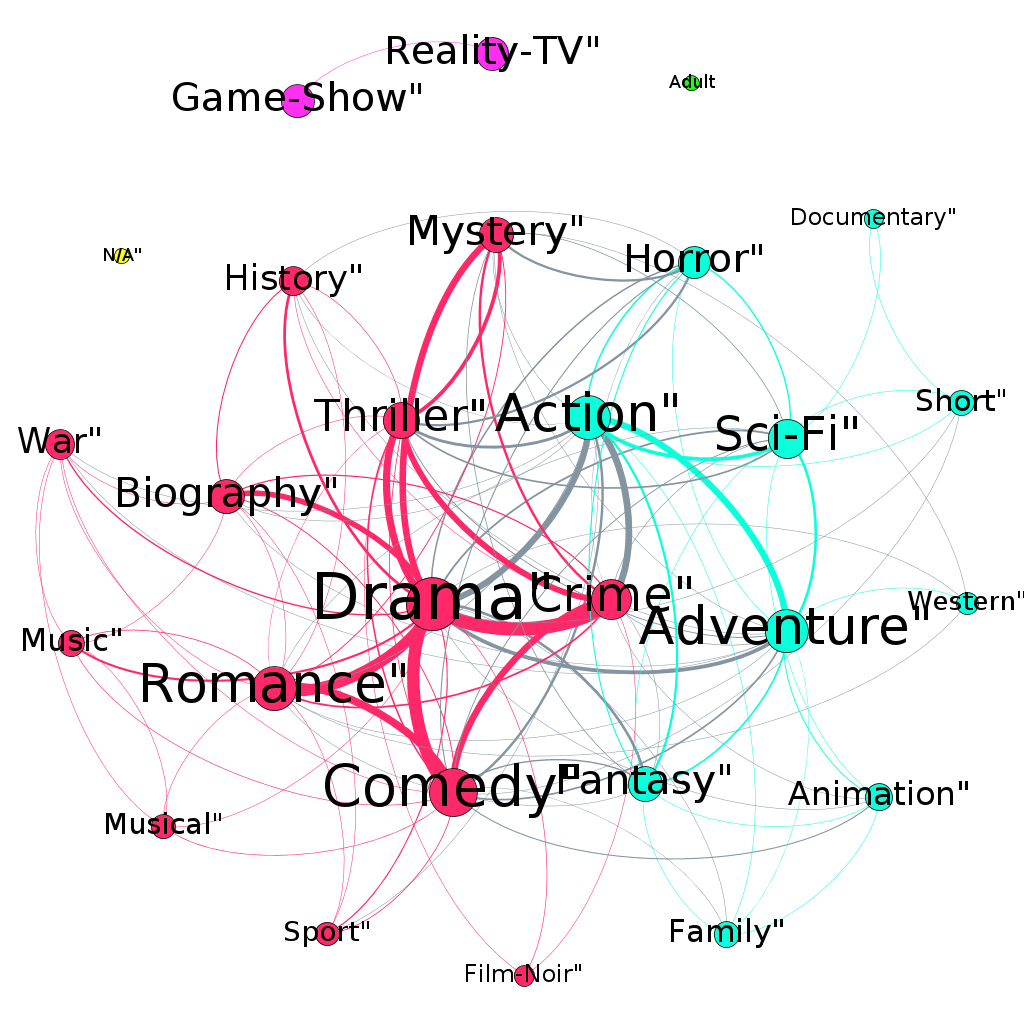
\includegraphics[width=0.65\textwidth]{../src/pre-processing/stats/results/CoocGenre.png}
\end{center}
\caption{Proximity between all genres}
\label{fig:coocGenre}
\end{figure}

\newpage
\subsubsection{Actors}
\label{subs:Actors}

As for directors, actors rankings that follow in Figures~\ref{fig:bestActors}~and~\ref{fig:worstActors}, once again, don't rate the talent of the actors mentioned.
They only represent how the ImDB users rated these actors' movies (that are in our dataset, if there are at least two movies for each actor in the dataset).
But they are quite consistent with global actors' fame.

\begin{figure}[!h]
\begin{center}
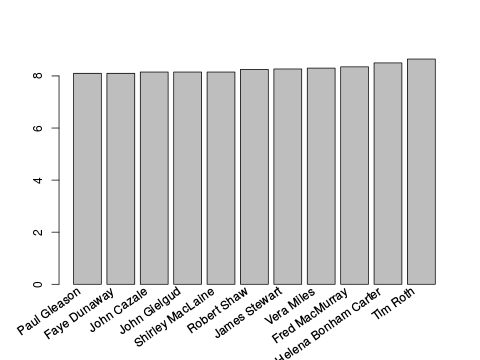
\includegraphics[width=0.70\textwidth]{../src/pre-processing/stats/results/bestActors.png}
\end{center}
\caption{Best-ranked actors}
\label{fig:bestActors}
\end{figure}

\begin{figure}[!h]
\begin{center}
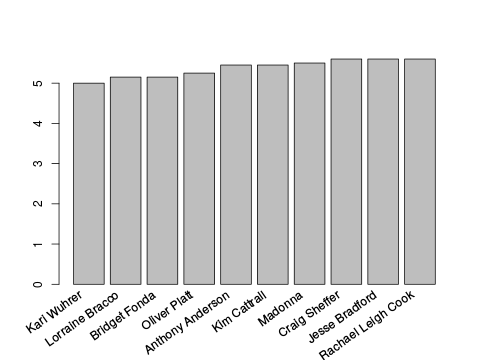
\includegraphics[width=0.70\textwidth]{../src/pre-processing/stats/results/worstActors.png}
\end{center}
\caption{Worst-ranked actors}
\label{fig:worstActors}
\end{figure}

\newpage
Figure~\ref{fig:coocActors} represents the network of actors playing together.
We can see that there is a very hudge connected component in the center of the graph, built around famous actors like Robert de Niro or Georges Clooney.
On the other hand, there is a lot of little independant cliques (for instance, there is one composed of Levar Burton, Patrick Stewart, Jonathan Frakes and Brent Spiner).
They represent actors who played together but not with other actors.
The theory behind this kind of graph is very strong\footnote{Thanks to \textit{Six Degrees of Kevin Bacon(}$https://en.wikipedia.org/wiki/Six\_Degrees\_of\_Kevin\_Bacon$\textit{)and many movie fans.}}.
Thus we know that this graph should be fully-connected, thanks to less-famous actors, who get minor roles in many movies.
Here, we only get the main actors for each movie when we query ImDB APIs. That makes the graph all the more so interesting to read.

\begin{figure}[!h]
\begin{center}
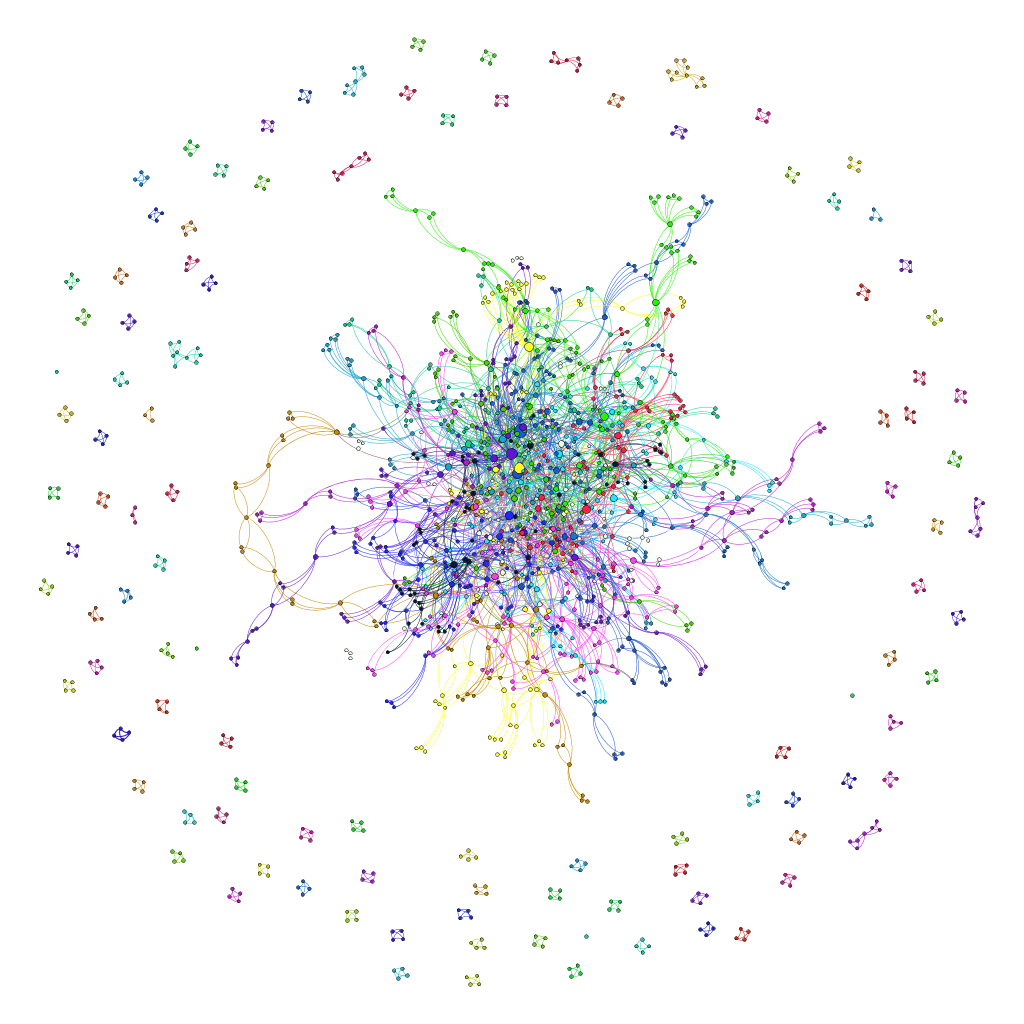
\includegraphics[width=1.1\textwidth]{../src/pre-processing/stats/results/CoocActors.png}
\end{center}
\caption{Network of actors playing together}
\label{fig:coocActors}
\end{figure}
